\section{MISSH}
\label{sec:MISSH}

Un ulteriore miglioramento all'algoritmo \acs{FSH} è stato raggiunto con \acs{MISSH}, sviluppato da \citeauthor*{mian2023missh} in \citetitle{mian2023missh} \cite{mian2023missh}. Come nel caso dell'Algoritmo~\ref{alg:FSH_multiple} relativo alla gestione di spaced seed multipli di \acs{FSH}, è stata dedicata particolare attenzione per lo sviluppo di un algoritmo che usasse la stessa idea di \acs{MISSH}, ma per un insieme di spaced seed.

Nell'articolo, gli autori propongono tre differenti approcci. Nella prima versione, chiamata \textbf{MISSH Multi}, vengono considerati contemporaneamente più spaced seed differenti, anche se l'hashing della sequenza di \acs{DNA} avviene in maniera indipendente per ciascun spaced seed. Infatti, per il calcolo di $h(x[i + Q_j])$ vengono sfruttati solamente gli hashing value precedenti e riferiti allo spaced seed $Q_j$. La differenza sostanziale con l'algoritmo \acs{ISSH} sta nel fatto che la hashing matrix è costruita per colonne, come illustrato in Figura~\ref{fig:issh_multi}. La convenienza sta nel fatto che l'ultimo carattere di ogni $Q$-gram, che viene sempre letto per la prima volta, appartiene a tutti gli hashing value a causa della definizione \ref{eq:spaced_kmer} di spaced seed data a pagina~\pageref{eq:spaced_kmer}. La lettura e la codifica del carattere vengono effettuate un'unica volta e sono valide per tutto il set di spaced seed.

\begin{figure}[!ht]
	\centering
	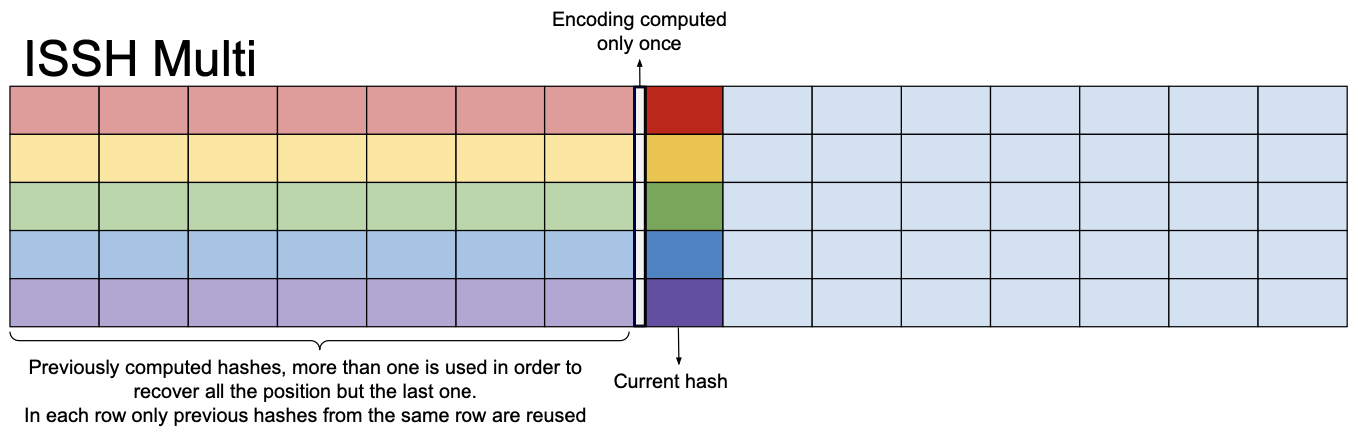
\includegraphics[width=0.85\linewidth]{images/issh_multi}
	\caption{A schematic representation of the ISSH Multi approach. The rows of the matrix represent the different spaced seeds, while the columns represent the position of the sequence where to compute the hash. \cite{mian2023missh}.}
	\label{fig:issh_multi}
\end{figure}

Il secondo approccio, \textbf{MISSH Multi Column}, si basa sull'approccio precedente e lo migliora introducendo un nuovo grado di libertà: in questo caso viene concesso di recuperare posizioni non solo da precedenti hashing value relativi allo stesso spaced seed, ma anche da spaced seed differenti da quello attualmente in considerazione. Una descrizione schematica può essere trovata in Figura~\ref{fig:issh_multi_column}.

\begin{figure}[!ht]
	\centering
	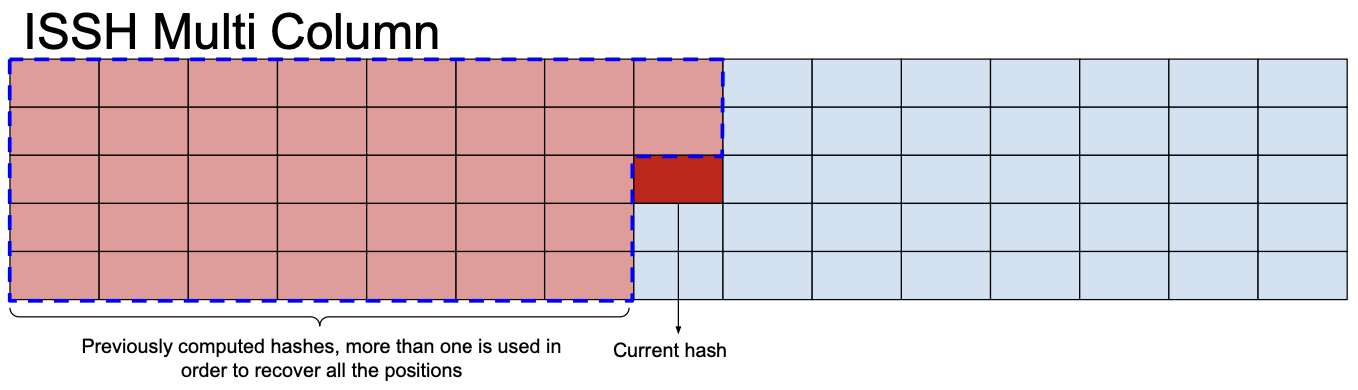
\includegraphics[width=0.85\linewidth]{images/issh_multi_column}
	\caption{A schematic representation of the ISSH Multi Column approach. The rows of the matrix represent the different spaced seeds, while the columns represent the position of the sequence where to compute the hash. \cite{mian2023missh}.}
	\label{fig:issh_multi_column}
\end{figure}

To compute a generic hash $h_{i,\; j}$, where $i$ is the index of the $Q$-gram to be hashed and $j$ is the index of the spaced seed, the algorithm searches for the hash $h_{n,\; m}$ that allows to recover most positions among all previously computed hashes. The condition that $h_{n,\; m}$ needs to satisfy in order to be used by $h_{i,\; j}$ is \begin{equation}\label{eq:issh_multi_column_condition}
	(n < i \textbf{ or } (n = i \textbf{ and } m < j)) \textbf{ and } n \geq 0.
\end{equation}
In order to extract symbols from $h_{n,\; m}$ to be reused in the new hash $h_{i,\; j}$ is defined a mask $Mask(j,\; n,\; m,\; l)$ that filters the appropriates positions.

\begin{algorithm}[!ht]
	\caption{ISSH Multi Column}
	\label{alg:ISSH_multi_column}
	\For{$i \gets 0$ \KwTo $|x| - s(Q)$}{
		\ForAll{$Q_j \in \vec{Q}$}{
			$h_{i,\; j} \gets 0$\;
			\While{missing positions can be recovered from available hashes}{
				$(n,\; m,\; l) \gets $ such that condition \ref{eq:issh_multi_column_condition} holds \KwAnd $h_{n,\; m}$ with $l$ shifts allows to recover the highest number of missing positions.\;
				$h_{i,\; j} \gets h_{i,\; j}$ \KwOr $((h_{n,\; m} >\!> (l \cdot \log_2 |\mathcal{A}|)$ \KwAnd $Mask(j,\; n,\; m,\; l))$\;
			}
			\If{there are still missing positions}{
				add missing encodings to $h_{i,\; j}$\;
			}
		}
	}
\end{algorithm}

Questo algoritmo presenta un notevole vantaggio perché riduce significativamente il numero di operazioni di codifica necessarie durante la fase transitoria. Innanzitutto, durante questa fase, il numero di operazioni di codifica è molto inferiore: anche l'hashing del primo $Q$-gram del secondo spaced seed ha già la possibilità di recuperare posizioni fin dal primo hash, cosa che non era possibile in precedenza. Inoltre, la funzione di codifica viene utilizzata solo una volta per ogni carattere nella sequenza, anche durante la fase transitoria. Questo approccio permette un notevole miglioramento nei tempi di calcolo rispetto all'algoritmo ISSH Multi. La possibilità di recuperare posizioni fin dal primo hash del secondo spaced seed significa che l'algoritmo può iniziare a ottenere risultati utili prima, migliorando l'efficienza complessiva. Infine, l'algoritmo ottimizza l'uso delle risorse computazionali, riducendo il carico di lavoro e permettendo un'elaborazione più rapida e meno dispendiosa in termini di tempo.

Infine, il terzo metodo, chiamato \textbf{ISSH Multi Row}, segue lo schema precedente invertendo l'ordine con cui riempie la hashing matrix. Riempiendola per righe è possibile recuperare posizioni anche dagli hash che sono stati calcolati in precedenza con uno spaced seed differente.

To compute a generic hash $h_{i,\; j}$, the algorithm searches for the hash $h_{n,\; m}$ that allows to recover most positions among all previously computed hashes. The condition that $h_{n,\; m}$ needs to satisfy in order to be used by $h_{i,\; j}$ is \begin{equation}\label{eq:issh_multi_row_condition}
	(m < j \textbf{ or } (m = j \textbf{ and } n < i)) \textbf{ and } 0 \leq n \leq |x| - s(Q).
\end{equation}

The schematic description can be found in Figure~\ref{fig:issh_multi_row}.

\begin{figure}[!ht]
	\centering
	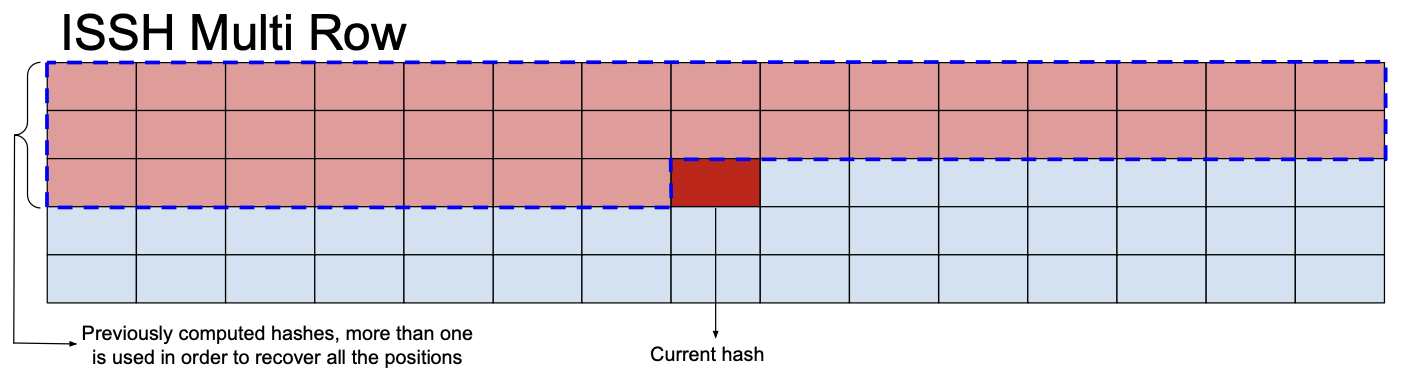
\includegraphics[width=0.85\linewidth]{images/issh_multi_row}
	\caption{A schematic representation of the ISSH Multi Row approach. The rows of the matrix represent the different spaced seeds, while the columns represent the position of the sequence where to compute the hash. \cite{mian2023missh}.}
	\label{fig:issh_multi_row}
\end{figure}

Questo altro algoritmo presenta vantaggi distinti derivanti dalla sua struttura e dalla gestione delle fasi transitorie. In particolare, l'introduzione di hash successivi, insieme a quelli precedenti, comporta una significativa modifica della fase transitoria. Questi hash sono generati dagli overlap dei spaced seed posizionati più a destra della posizione corrente. Tale approccio comporta la presenza di due fasi transitorie, una all'inizio e una alla fine della sequenza di DNA. Questo è dovuto al fatto che gli hash "a destra" calcolati durante il pre-processamento alla fine non saranno disponibili, proprio come gli hash "a sinistra" non erano inizialmente disponibili. Inoltre, ci si aspetta che questo metodo abbia una performance migliore su sequenze più lunghe. La presenza di due fasi transitorie e la gestione degli hash "a destra" lo rendono più efficiente nella gestione di sequenze di lunghezza maggiore. Di conseguenza, è in grado di fornire risultati migliori e più affidabili rispetto ad altri metodi, specialmente quando la lunghezza delle sequenze è un fattore critico da considerare.
